\section{Estructura de la base de datos}

% Incluye:
% - Una lista de variables con sus nombres, unidades y descripciones
% - Qué tipo de datos contiene cada campo (numérico, categórico, geográfico)
% - Cuántos registros hay, si hay valores faltantes, etc.
% Puedes presentar una tabla con:
% | Variable | Descripción | Unidad | Tipo de dato |

La base de datos se organiza bajo un modelo relacional normalizado que garantiza la integridad referencial y la trazabilidad de los datos. Todas las claves primarias (\textit{PK}) están definidas explícitamente y siguen una nomenclatura uniforme terminada en \texttt{\_id}, representando la granularidad del dato en cada nivel jerárquico. De igual forma, las claves foráneas (\textit{FK}) se encuentran activas y estrictamente validadas, cubriendo el 100\% de los valores no nulos y asegurando la ausencia de registros huérfanos.

El esquema se ha diseñado para ser evolutivo y auditable. Las relaciones principales (PK/FK) permanecen estables, mientras que las tablas son extensibles, permitiendo incorporar nuevas métricas sin comprometer la coherencia estructural. La tabla \texttt{meta\_variables} complementa esta arquitectura documentando el tipo, unidades, método de cálculo, rango esperado y fuente de cada variable, lo que facilita la trazabilidad analítica y la reproducibilidad de los resultados.

\subsection*{Panorama de entidades}

Las tablas se agrupan en dos conjuntos: \textbf{núcleo} y \textbf{catálogos}.  
El núcleo contiene las entidades troncales que almacenan la información principal del sistema, mientras que los catálogos definen dominios controlados para las variables categóricas, garantizando consistencia terminológica en toda la base de datos.

\paragraph{Núcleo}
\begin{itemize}
  \item \textbf{parcelas}: identifica la unidad espacial (\texttt{parcela\_id}) y almacena su geometría básica (coordenadas, superficie, elevación, pendiente, etc.). Es la entidad raíz del modelo.
  \item \textbf{parcela\_inventario}: describe el estado de cada parcela en un inventario determinado (\texttt{parcela\_id}, \texttt{inventario\_id}), incluyendo atributos edáficos y de contexto (p. ej., \texttt{nivel1\_id}, \texttt{textura\_id}).
  \item \textbf{parcela\_inventario\_especie}: detalla la presencia y condición de cada especie dentro de una parcela e inventario, incorporando descriptores de masa y tratamientos silvícolas.
  \item \textbf{parcela\_inventario\_especie\_cd}: describe las poblaciones arbóreas por parcela, especie y \emph{clase diamétrica} (\texttt{cd\_id}): n.º de pies (\texttt{npies}), área basimétrica (\texttt{abas}), volúmenes (\texttt{vcc}, \texttt{vsc}, \texttt{vle}), incrementos (\texttt{iavc}) y carbono (\texttt{ca}, \texttt{cr}).
  \item \textbf{parcela\_especie\_arbol}: caracteriza los pies mayores identificados por parcela y especie en el inventario cuarto. Recoge las caracteristicas particulares de cada pie como altura (\texttt{ht}), diámetros (\texttt{dn1} y \texttt{dn2}), ubicación respecto del centro de la parcela (\texttt{rumbo}, \texttt{distancia}), volumen (\texttt{vcc, vsc, vle}), incremento (\texttt{iavc}) y carbono (\texttt{ca, cr}).  
  \item \textbf{parcela\_inventario\_estacion}: almacena agregados climático-biofísicos por estación (\texttt{estacion\_id}) en la misma granularidad parcela–inventario, incluyendo variables como precipitación (\texttt{PR}) y temperatura (\texttt{T2M, SKT, STL*}), junto a índices de vegetación (NDVI, EVI, NDII, GNDVI).
  \item \textbf{especies} y \textbf{grupos}: recogen la información taxonómica y su clasificación jerárquica, estableciendo la relación entre especies individuales y grupos funcionales.
\end{itemize}

\paragraph{Catálogos}
Cada variable categórica posee una tabla de catálogo propia (\texttt{cat\_}), donde se definen los valores posibles y sus descripciones. Por ejemplo, \texttt{cat\_textura}, \texttt{cat\_nivel1}, \texttt{cat\_tratmasa} o \texttt{cat\_origen}. Todas siguen un patrón uniforme: la clave primaria es el identificador de la variable (\texttt{<variable>\_id}), y las tablas núcleo referencian este mismo campo como clave foránea. Esto permite mantener un dominio controlado y una semántica coherente en toda la base de datos.

\subsection*{Representación del esquema}

La Figura~\ref{fig:GWest_BBDD} muestra el esquema general de las tablas nucleares y sus principales relaciones. Este diagrama resume la estructura interna de la base de datos y su jerarquía de dependencias.

\begin{figure}[H]
  \centering
  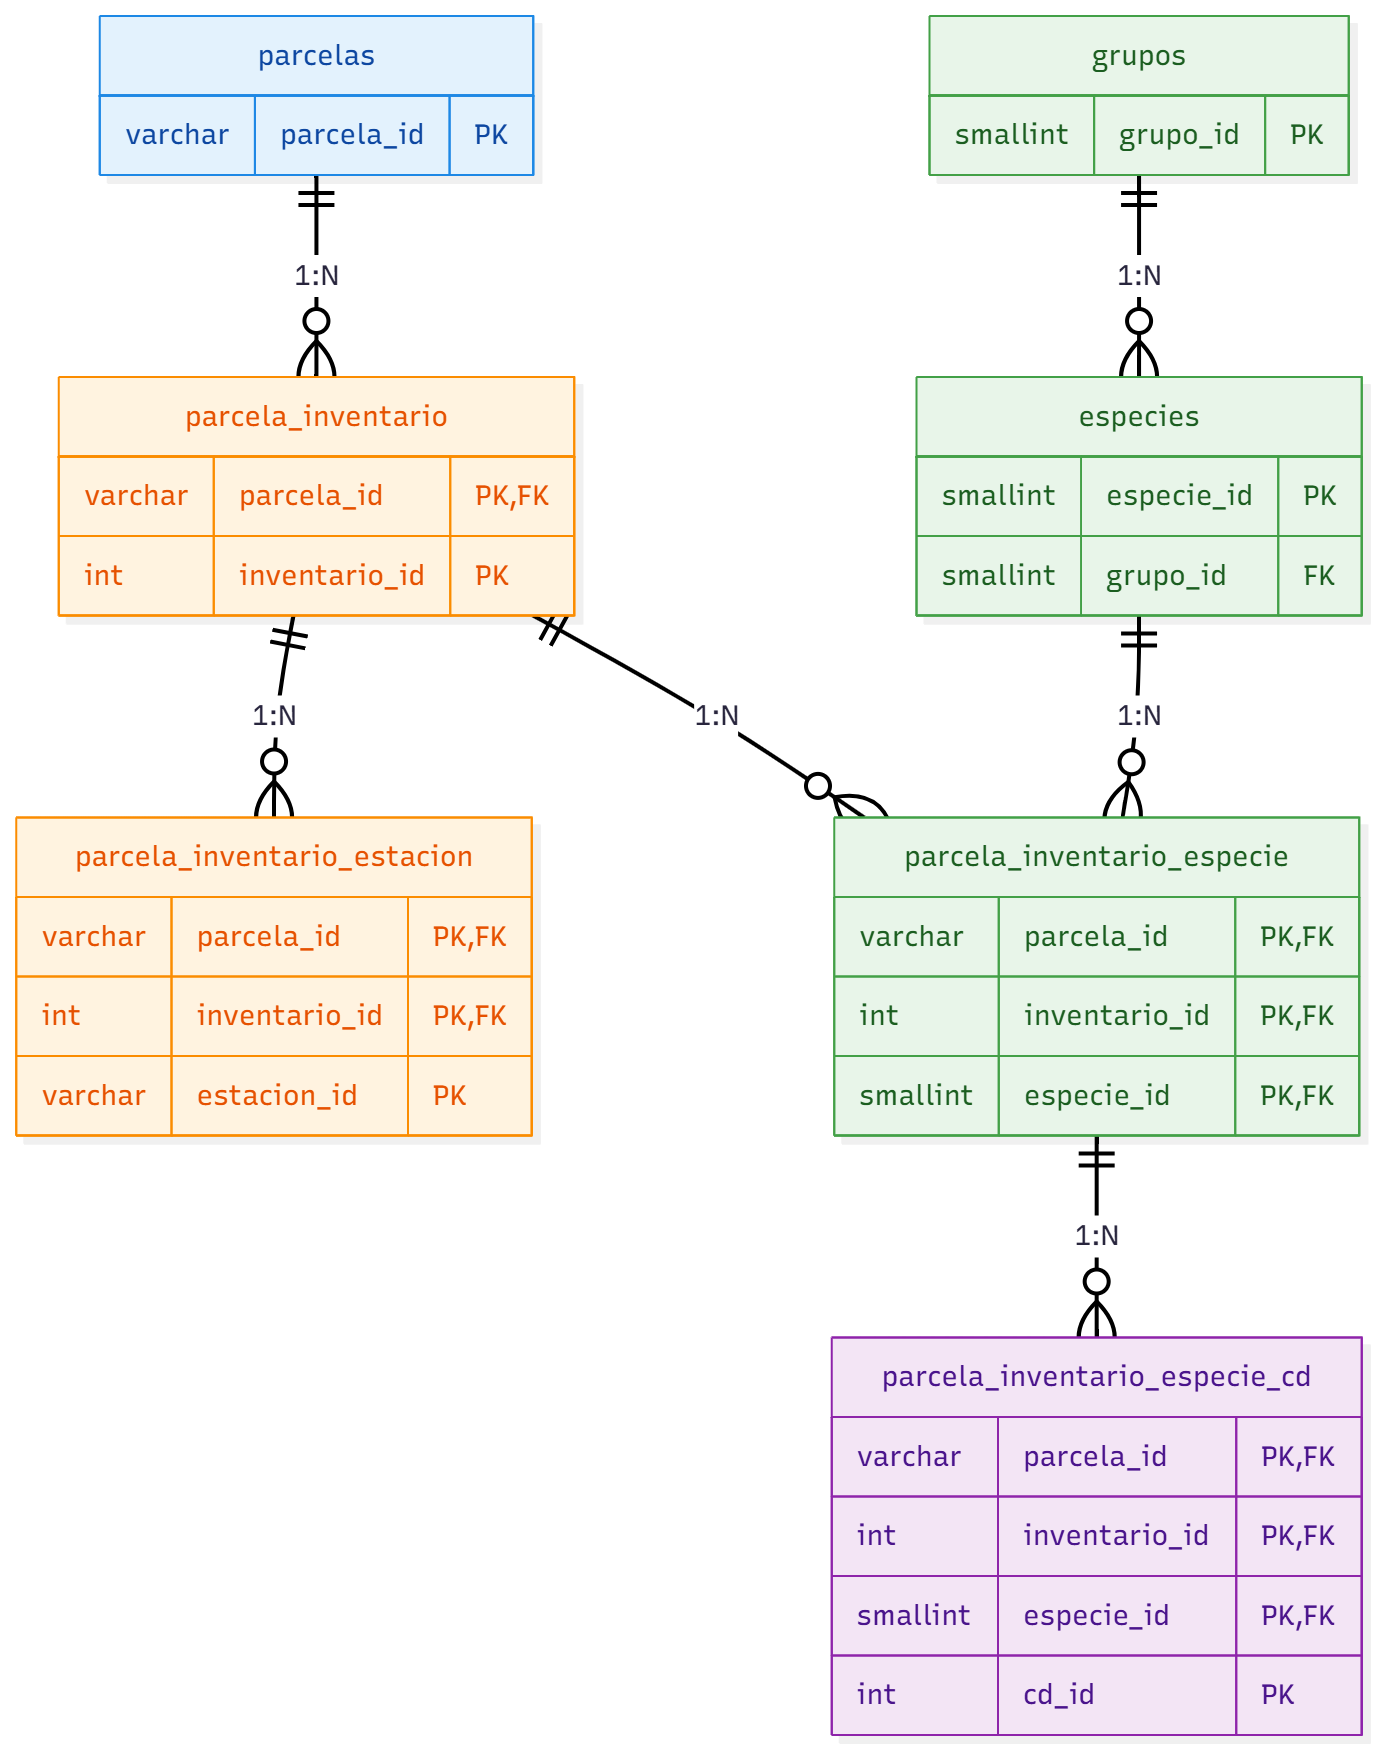
\includegraphics[width=0.9\textwidth]{figuras/Estrctr_BBDD_GWest.png}
  \caption{Esquema relacional de las tablas nucleares de la base de datos.}
  \label{fig:GWest_BBDD}
\end{figure}

\subsection*{Tipología de datos y convenciones}

Cada columna se tipifica en una de cuatro categorías:
\begin{itemize}
  \item \textbf{Numérico}: magnitudes continuas (p.\,ej., \texttt{npies}, \texttt{vcc}, \texttt{ndvi\_mean}, \texttt{elevacion}).
  \item \textbf{Categórico}: códigos discretos con dominio controlado mediante catálogos \texttt{cat\_*} (p.\,ej., \texttt{nivel1\_id}, \texttt{textura\_id}, \texttt{tratmasa\_id}).
  \item \textbf{Identificador}: claves primarias y foráneas terminadas en \texttt{\_id} (p.\,ej., \texttt{parcela\_id}, \texttt{inventario\_id}, \texttt{especie\_id}, \texttt{cd\_id}).
  \item \textbf{Geográfico}: coordenadas y derivados topográficos (\texttt{latitud}, \texttt{longitud}, \texttt{coorx}/\texttt{coory}, \texttt{pendiente}, \texttt{orientacion}).
\end{itemize}

Las variables satelitales y climáticas usan convenciones de \emph{valores especiales} para datos no disponibles o enmascarados por calidad (\texttt{NA}); los rangos esperados se documentan en \texttt{meta\_variables}. Todas las claves categóricas referencian explícitamente su catálogo homólogo (\texttt{<variable>\_id} $\rightarrow$ \texttt{cat\_<variable>(<variable>\_id)}).

\subsection*{Cardinalidad y completitud}

El volumen actual por tabla es:
\begin{center}
\begin{tabular}{l r}
\toprule
\textbf{Tabla} & \textbf{Número de registros} \\
\midrule
\texttt{parcelas} & 52{,}298 \\
\texttt{parcela\_inventario} & 147{,}995 \\
\texttt{parcela\_inventario\_especie} & 417{,}119 \\
\texttt{parcela\_inventario\_especie\_cd} & 1{,}191{,}070 \\
\texttt{parcela\_especie\_arbol} & 855{,}860 \\
\texttt{parcela\_inventario\_estacion} & 470{,}056 \\
\texttt{especies} & 195 \\
\texttt{grupos} & 33 \\
\bottomrule
\end{tabular}
\end{center}

Las \textit{FK} estructurales están activas y cubren el 100\,\% de los valores no nulos (sin huérfanos). La completitud de campos numéricos puede verse afectada por enmascaramientos de calidad en series satelitales/climáticas, registrados como \texttt{NA} según \texttt{meta\_variables}. Las variables categóricas presentan dominios cerrados controlados por sus catálogos.

\subsection*{Diccionario resumido de variables (núcleo)}
\small
\setlength{\LTcapwidth}{\textwidth}
\begin{longtable}{p{3.2cm} p{7.6cm} p{2.4cm} p{2.4cm}}
\caption{Resumen de variables principales por entidad. El diccionario completo se encuentra documentado en \texttt{meta\_variables}.}\\
\toprule
\textbf{Variable} & \textbf{Descripción} & \textbf{Unidad} & \textbf{Tipo de dato} \\
\midrule
\endfirsthead
\toprule
\textbf{Variable} & \textbf{Descripción} & \textbf{Unidad} & \textbf{Tipo de dato} \\
\midrule
\endhead
\midrule
\multicolumn{4}{r}{\emph{Continúa en la siguiente página}} \\
\midrule
\endfoot
\bottomrule
\endlastfoot

\multicolumn{4}{l}{\textbf{parcelas}} \\
\texttt{parcela\_id} & Identificador único de parcela (IFN). & -- & Identificador \\
\texttt{latitud}, \texttt{longitud} & Coordenadas geográficas (WGS84). & ° & Geográfico \\
\texttt{coorx}, \texttt{coory} & Coordenadas UTM; \texttt{huso} especifica zona. & m (UTM) & Geográfico \\
\texttt{elevacion} & Cota sobre el nivel del mar (NASADEM). & m & Numérico \\
\texttt{pendiente} & Inclinación del terreno. & ° & Numérico \\
\texttt{orientacion} & Orientación del terreno (0–360). & ° & Numérico \\
\texttt{presencia\_id} & Presencia en IFN $\rightarrow$ \texttt{cat\_presencia}. & -- & Categórico \\
\texttt{tipsuelo1\_id}, \texttt{tipsuelo2\_id}, \texttt{tipsuelo3\_id} & Tipos de suelo $\rightarrow$ \texttt{cat\_tipsuelo*}. & -- & Categórico \\
\texttt{rocosidad\_id} & Rocosidad $\rightarrow$ \texttt{cat\_rocosidad}. & -- & Categórico \\
\texttt{radio}, \texttt{superficie} & Radio de parcela y superficie derivada. & m; ha & Numérico \\
\addlinespace

\multicolumn{4}{l}{\textbf{parcela\_inventario}} \\
\texttt{parcela\_id}, \texttt{inventario\_id} & Clave compuesta (parcela-inventario). & -- & Identificador \\
\texttt{ano} & Año de apeo. & año & Numérico \\
\texttt{nivel1\_id}, \texttt{nivel2\_id} & Morfoestructura. $\rightarrow$ \texttt{cat\_nivel*}. & -- & Categórico \\
\texttt{textura\_id} & Textura de suelo $\rightarrow$ \texttt{cat\_textura}. & -- & Categórico \\
\texttt{merosiva\_id} & Manifestaciones erosivas $\rightarrow$ \texttt{cat\_merosiva}. & -- & Categórico \\
\texttt{matorg\_id} & Materia orgánica $\rightarrow$ \texttt{cat\_matorg}. & -- & Categórico \\
\texttt{modcomb\_id} & Modelo de combustible $\rightarrow$ \texttt{cat\_modcomb}. & -- & Categórico \\
\texttt{disesp\_id} & Distribución espacial $\rightarrow$ \texttt{cat\_disesp}. & -- & Categórico \\
\texttt{comesp\_id} & Composición específica $\rightarrow$ \texttt{cat\_comesp}. & -- & Categórico \\
\texttt{fccarb}, \texttt{fcctot} & Fracción de cabida cubierta (árboles). & \% & Numérico \\
\addlinespace

\multicolumn{4}{l}{\textbf{parcela\_inventario\_especie}} \\
\texttt{parcela\_id}, \texttt{inventario\_id}, \texttt{especie\_id} & Clave compuesta (parcela-inventario-especie). & -- & Identificador \\
\texttt{ocupa} & Grado de ocupación de la especie. & (0--10) & Numérico \\
\texttt{estado\_id} & Estado de desarrollo. $\rightarrow$ \texttt{cat\_estado}. & -- & Categórico \\
\texttt{fpmasa\_id} & Forma principal de masa $\rightarrow$ \texttt{cat\_fpmasa}. & -- & Categórico \\
\texttt{tratmasa\_id} & Tratamientos selvícolas $\rightarrow$ \texttt{cat\_tratmasa}. & -- & Categórico \\
\texttt{orgmasa1\_id} & Origen de masa (IFN3/4)$\rightarrow$ \texttt{cat\_orgmasa1}. & -- & Categórico \\
\texttt{masa\_id} & Clasificación de masa $\rightarrow$ \texttt{cat\_masa}. & -- & Categórico \\
\texttt{origen\_id} & Origen de la masa (IFN2) $\rightarrow$ \texttt{cat\_origen}. & -- & Categórico \\
\addlinespace

\multicolumn{4}{l}{\textbf{parcela\_inventario\_especie\_cd}} \\
\texttt{parcela\_id}, \texttt{inventario\_id}, \texttt{especie\_id} & Clave compuesta ( parcela-inventario-especie-cd). & -- & Identificador \\
\texttt{cd\_id} & Clase diamétrica (CD) reglamento IFN. & cm & Numérico discreto \\
\texttt{npies} & Número de pies. & pies/ha & Numérico \\
\texttt{abas} & Área basimétrica. & m$^{2}$/ha & Numérico \\
\texttt{vcc}, \texttt{vsc}, \texttt{vle} & Volúmenes (con/sin corteza; leñas). & m$^{3}$/ha & Numérico \\
\texttt{iavc} & Incremento anual del volumen con corteza. & m$^{3}$/ha$\cdot$año & Numérico \\
\texttt{ca}, \texttt{cr} & Carbono aéreo y radical. & tC/ha & Numérico \\
\texttt{ht} & Altura media (modelo CatBoost). & m & Numérico \\
\texttt{carbono\_bruto} & Carbono total estimado (alometrías). & t & Numérico \\
\addlinespace

\multicolumn{4}{l}{\textbf{parcela\_especie\_arbol}} \\
\texttt{parcela\_id}, \texttt{especie\_id} & Clave compuesta (parcela–especie–árbol). & -- & Identificador \\ 
\texttt{arbol\_id} & Identificador del árbol dentro de parcela y especie. & -- & Entero \\ 
\texttt{rumbo} & Rumbo desde el centro de la parcela al árbol. & grados centesimales & Numérico \\ 
\texttt{distancia} & Distancia desde el centro de la parcela al árbol. & m & Numérico \\ 
\texttt{cd} & Clase diamétrica (reglamento IFN). & cm & Numérico discreto \\ 
\texttt{ht} & Altura total del árbol inventariado. & m & Numérico \\ 
\texttt{dn1}, \texttt{dn2} & Diámetros normales perpendiculares. & mm & Numérico \\ 
\texttt{abas} & Área basimétrica del pie medido. & m$^{2}$ & Numérico \\ 
\texttt{iavc} & Incremento anual del volumen con corteza. & dm$^{3}$/año & Numérico \\ 
\texttt{vcc}, \texttt{vsc}, \texttt{vle} & Volúmenes (con corteza, sin corteza, leñas). & dm$^{3}$ & Numérico \\ 
\texttt{ca}, \texttt{cr} & Carbono aéreo y radical del árbol. & t & Numérico \\
\addlinespace

\multicolumn{4}{l}{\textbf{parcela\_inventario\_estacion}} \\
\texttt{parcela\_id}, \texttt{inventario\_id}, \texttt{estacion\_id} & Clave compuesta (agregado estacional). & -- & Identificador \\
\texttt{PR\_*} & Estadísticos de precipitación (mean, max, min, std, sum). & mm/(m$^2\cdot$día), mm/m$^2$ & Numérico \\
\texttt{T2M\_*}, \texttt{SKT\_*} & Aire 2\,m y temperatura superficial (mean, max, min, std). & °C & Numérico \\
\texttt{STL1\_*}--\texttt{STL4\_*} & Temperatura del suelo por niveles (mean, max, min, std). & °C & Numérico \\
\texttt{NDVI\_*}, \texttt{EVI\_*}, \texttt{NDII\_*}, \texttt{GNDVI\_*} & Índices de vegetación (max, mean, median, min, std). & adimensional & Numérico \\
\addlinespace

\multicolumn{4}{l}{\textbf{especies} y \textbf{grupos}} \\
\texttt{especie\_id} & Identificador de especie IFN. & -- & Identificador \\
\texttt{nombre}, \texttt{sinonimia} & Denominación IFN y sinónimos. & -- & Texto \\
\texttt{tipo\_especie} & 0\,= conífera; 1\,= frondosa. & -- & Categórico \\
\texttt{grupo\_id} & Grupo funcional $\rightarrow$ \texttt{grupos}. & -- & Identificador \\
\texttt{grupos.nombregrupo} & Nombre del grupo. & -- & Texto \\
\end{longtable}
\normalsize
\subsection*{Calidad de datos y valores faltantes}

Las validaciones automáticas garantizan:
\begin{enumerate}
  \item \textbf{Integridad referencial}: todas las \textit{FK} (\texttt{parcela\_id}, \texttt{inventario\_id}, \texttt{especie\_id} y catálogos \texttt{cat\_*}) están resueltas sin registros huérfanos.
  \item \textbf{Rangos y dominios}: se verifican contra \texttt{rango\_esperado} y \texttt{valores\_especiales} de \texttt{meta\_variables}.
  \item \textbf{Faltantes}: en variables derivadas de teledetección o reanálisis es esperable \texttt{NA} por enmascaramiento de nubes o cobertura temporal; estos valores se excluyen de los estadísticos agregados o se imputan explícitamente según el análisis.
\end{enumerate}
